
%%%%%%%%%%%%%%%%%%%%%%%%%%%%%%%%%%%%%%%%%%%%%%%%%%%%%%%%%%%%%%%%%%%%%%%%%%%%%%%%%%
%%% Platform Description
%%% Add sample data from cameras and lidar
%%% Section 1 : Hardware Overview
%%%		SubSection 1.1 : Pertinent Nao Statistics (and how things talk to each other)
%%% 	SubSection 1.2 : Pertinent Lidar Statistics
%%%		SubSection 1.3 : Design Requirements for Lidar Mount and Description
%%% Section 2 : Software Framework
%%%		SubSection 2.1 : NaoQi and qibuild Overview
%%% 	SubSection 2.2 : Custom Library Framework
%%%		SubSection 2.3 : User Operation
%%%
%%%%%%%%%%%%%%%%%%%%%%%%%%%%%%%%%%%%%%%%%%%%%%%%%%%%%%%%%%%%%%%%%%%%%%%%%%%%%%%%%%
\chapter{Platform}\label{ch:platform}

For this thesis we used the Nao as the mobile platform. Aldebaran makes him.
He's a cool little robot and he allows us to explore both things we wanted to 
look at which were navigation and gaiting. He's mobile, small, ``cost-effective''
and has a good API that we can use to do lower-level control of things when we want to, 
and abstract ourselves from it when we don't want to.
The small size means he's easy to work with.

There's definitely some more opening paragraph to be written here about the Nao.
Probably say something about why he's useful to investigate crawling.
No one's going to send Nao into a disaster zone or anything but he's not too
far off from robots that you would send in and we don't have to spend all the 
money or build a new lab to work with him. You can do lot's of simulations, 
but in the end you still have to test on a real robot.

While the Nao is cool and all, the sonar sensors just don't cut it for what we want to do.
Lucky, Nao comes with a USB port and uses x86 and linux so it's relatively
straightforward to add new things to him. Therefore, we added a better distance sensor.
Specifically we added the Hokuyo URG-04LX-UG01.
It's a good Lidar because it has a respectable range, good angular resolution,
``cost-effective'', and is kinda lightweight. Using this sensor we could do mapping 
if we wanted to which means this system is extensible to the broader challeges 
of the overall navigation problem such as SLAM\@. Using the Lidar we'll be able to 
get enough information to do the job we need to.

While it's easy to plug a USB cable into Nao's head, you still have to stick the Lidar somewhere.
Nao doesn't have mount points that make it easy to add new hardware.
Given that we have a nifty 3D printer (and I know Solidworks) we designed up a little suit of
armor for Nao with a big stick coming out of it that we could mount the Lidar to, above his head.
This works but the new dynamics destabilize Nao's default gait at certain speeds. 
This doesn't mess with the navigation algorithm, but to increase the speed this will have to be dealt with,
either by changing the rig or \ldots using the arms to counterbalance the new inertial forces as
part of the walking gait.

\begin{figure}
\centering
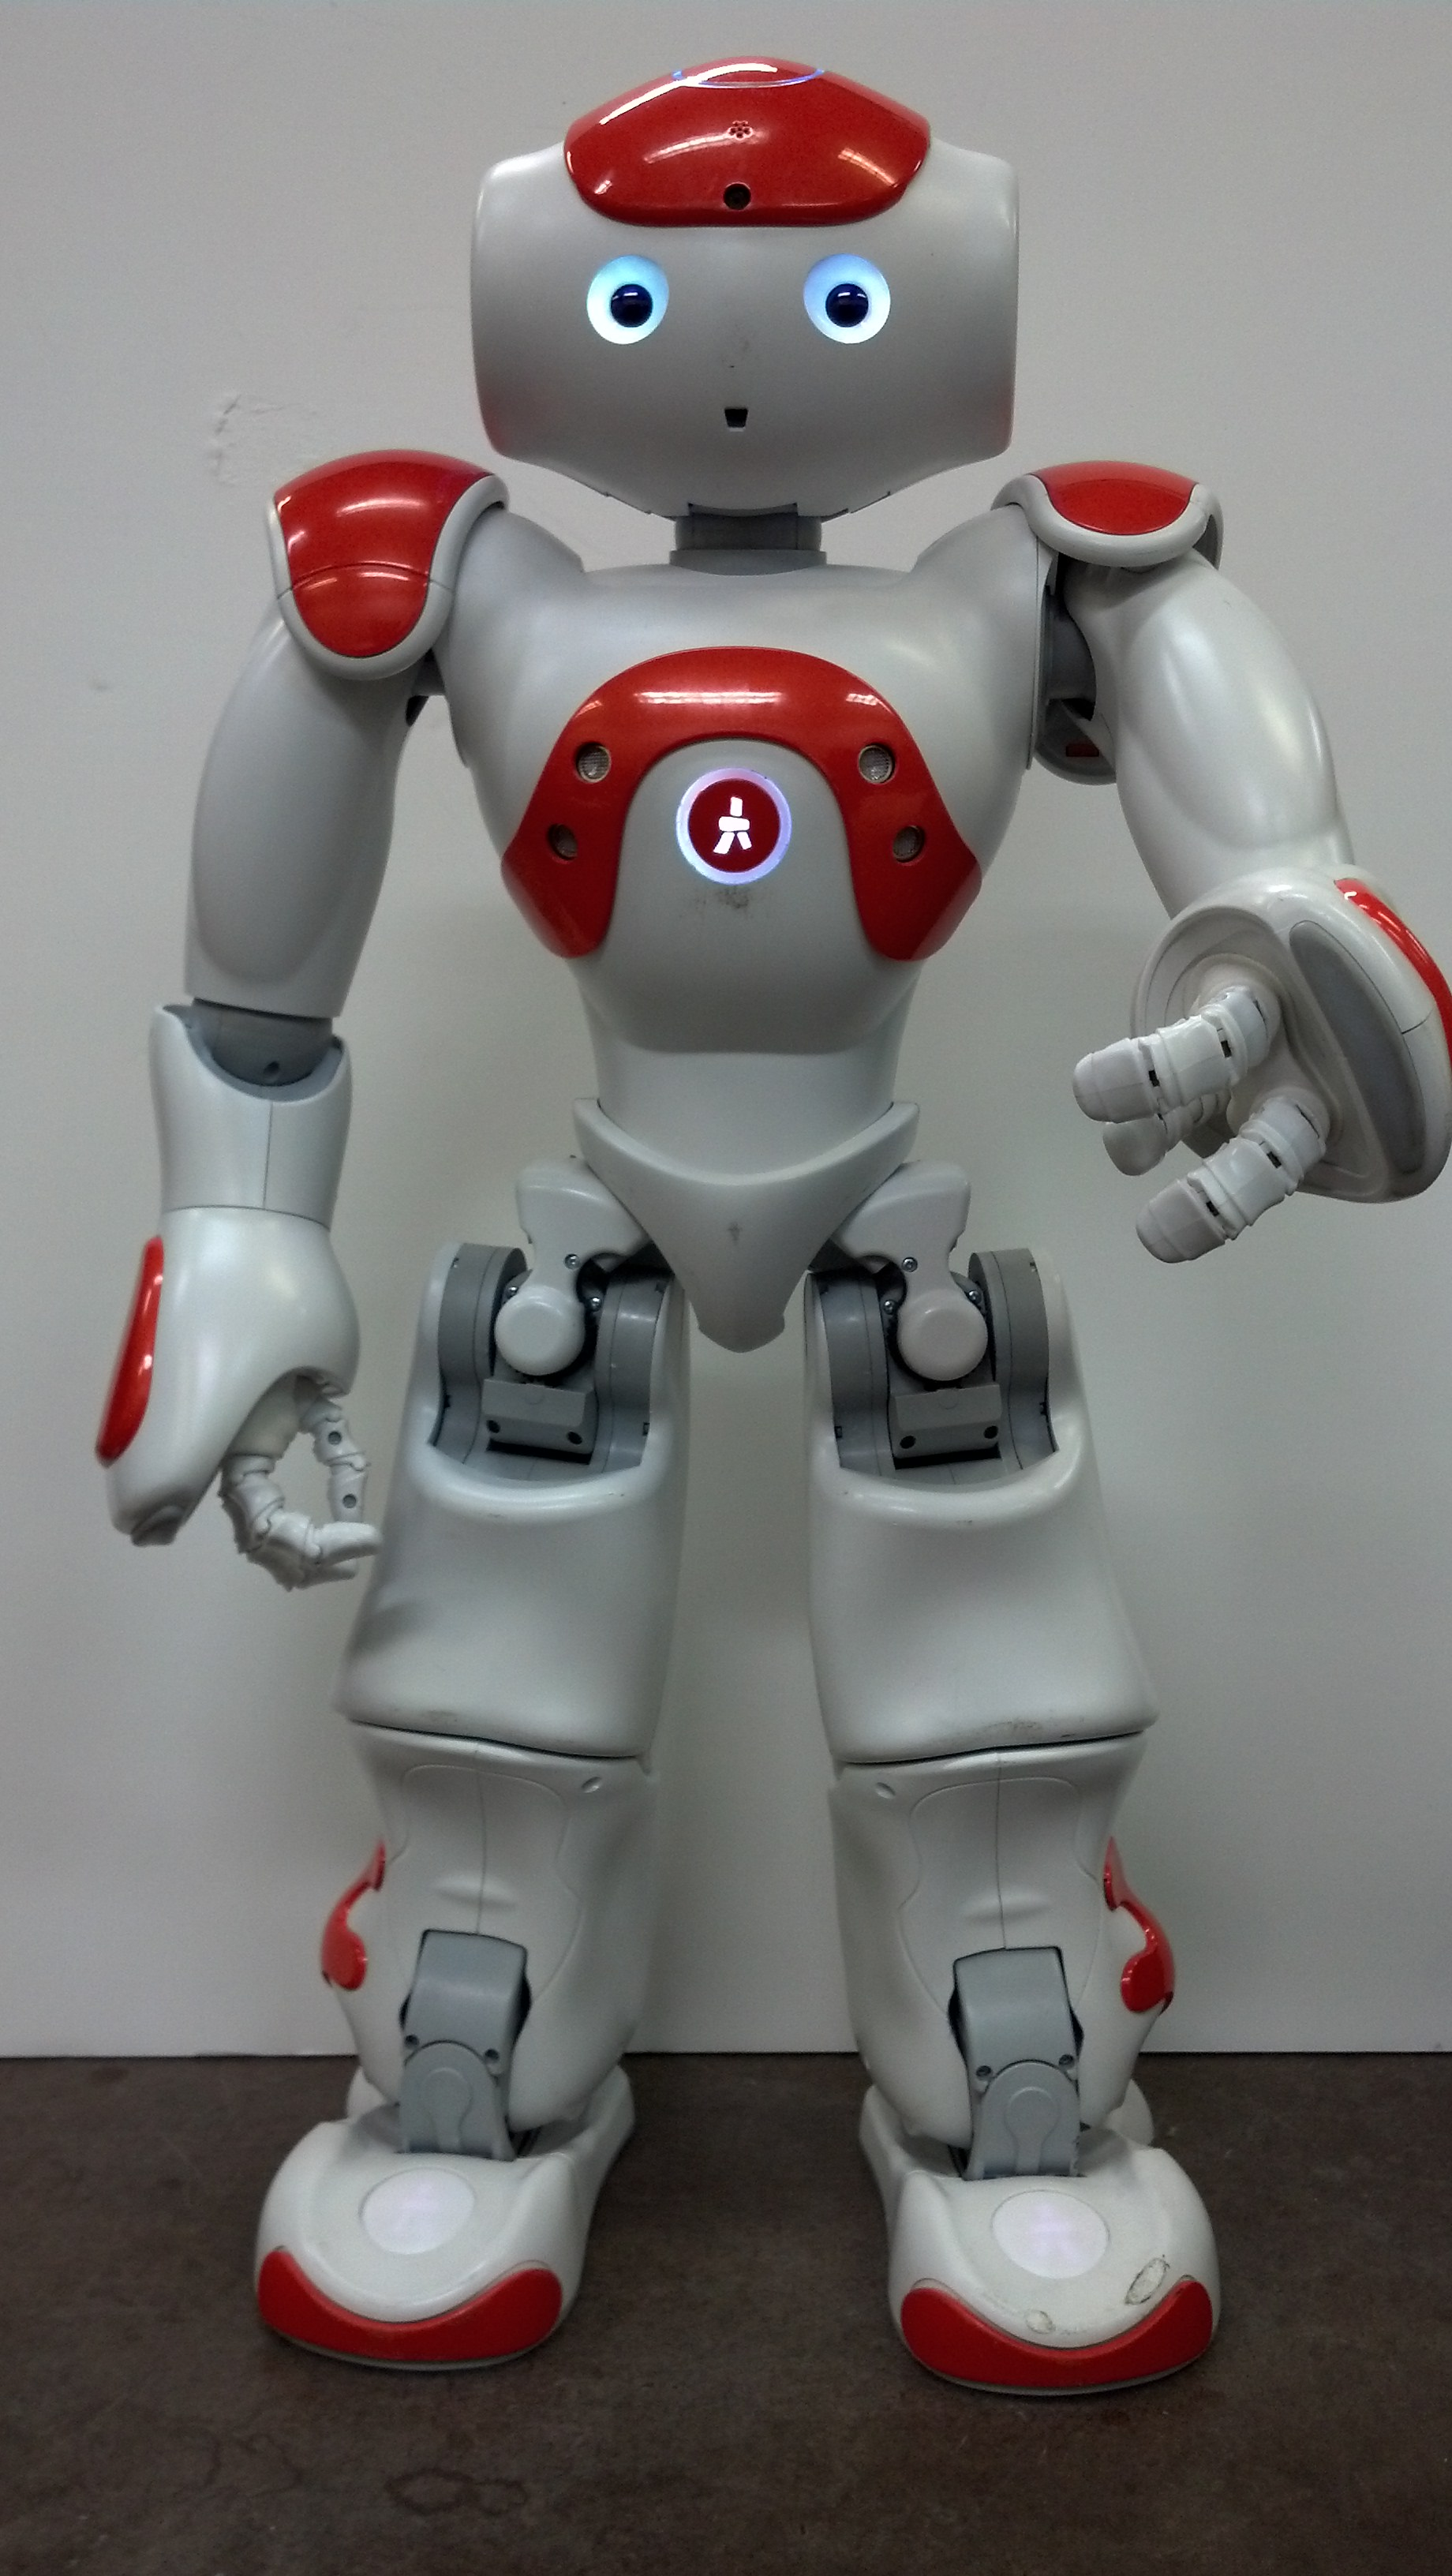
\includegraphics[height=0.4\textheight]{nao_coronal1.jpg}
\caption{Nao at CRRL.}
\label{fig:crrl_nao_coronal1}
\end{figure}

\begin{figure}
\centering
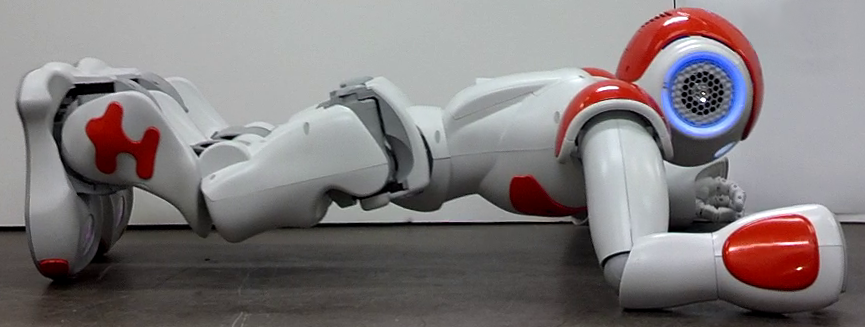
\includegraphics[width=\textwidth]{White_Background/apex_cropped.png}
\caption{Nao in crawling pose.}
\label{fig:crrl_nao_apex1}
\end{figure}

\begin{figure}
\centering
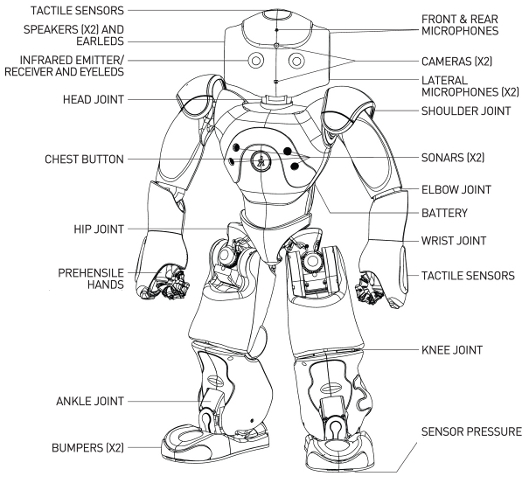
\includegraphics[width=\textwidth]{nao_diagrams/nao_h25_pres.png}
\caption{Nao features.}
\label{fig:nao_features1}
\end{figure}

\begin{figure}
\centering
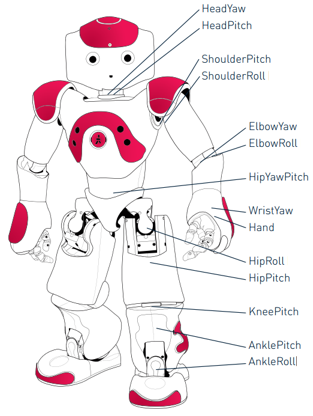
\includegraphics[height=0.4\textheight]{nao_diagrams/hardware_motortype_h25V5.png}
\caption{Nao joints.}
\label{fig:nao_joints1}
\end{figure}

\begin{figure}
\centerline{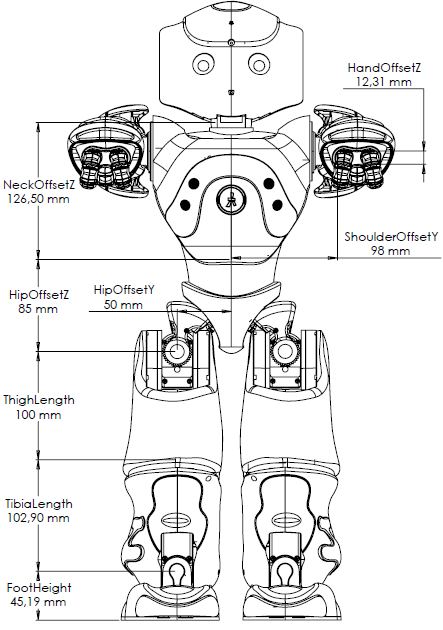
\includegraphics[width=0.45\textwidth]{nao_diagrams/hardware_lengthfront_3.3.png}
            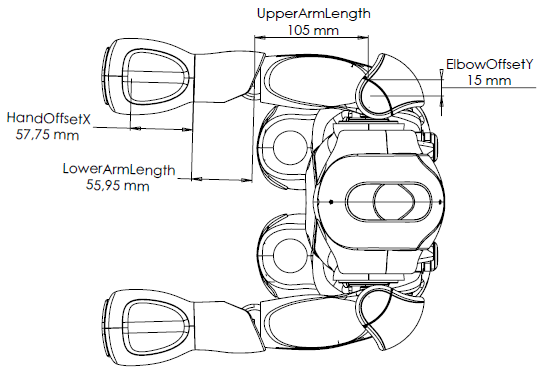
\includegraphics[width=0.55\textwidth]{nao_diagrams/hardware_lengthup_3.3.png}
}
\caption{Nao link lengths.}
\label{fig:nao_link_lengths1}
\end{figure}

\begin{figure}
\centering
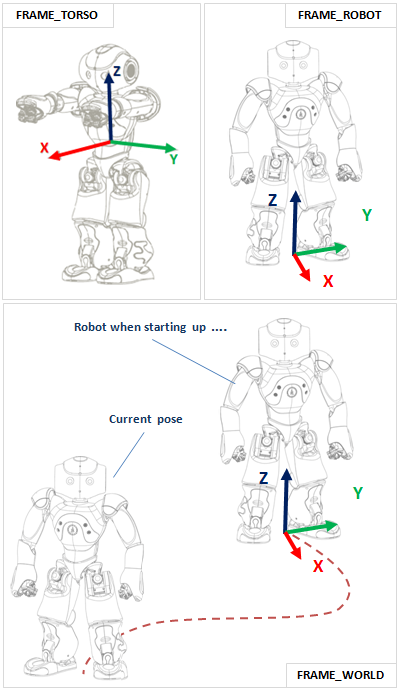
\includegraphics[height=0.75\textheight]{nao_diagrams/frame_definition_combo.png}
\caption{Nao frames.}
\label{fig:nao_frames1}
\end{figure}

\begin{figure}
\centerline{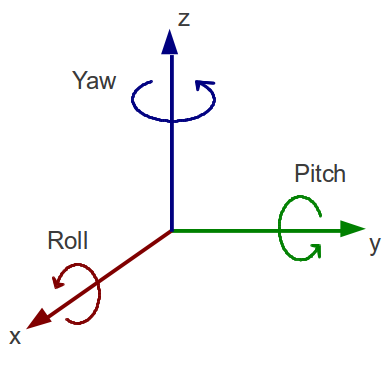
\includegraphics[width=0.5\textwidth]{nao_diagrams/rollPitchYaw.png}
}
\caption{Definition of roll pitch and yaw.}
\label{fig:nao_rpy_def1}
\end{figure}

\section{Hardware Overview}
Ok so, three pieces of hardware here, the Nao, the Lidar, and the mount.
Technically, all you need is the Nao since it is a mobile base with distance sensors but the sonars
don't do that great so we added the Lidar, and since there's no where to screw it down we designed a mount.

\begin{figure}
\centering
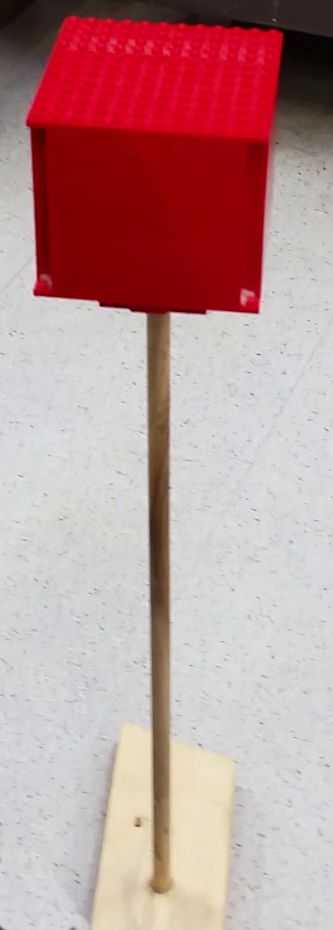
\includegraphics[height=0.4\textheight]{red_cube1.png}
\caption{Figure showing red cube the Nao tracked.}
\label{fig:red_cube1}
\end{figure}

\subsection{Nao Hardware}
Nao is a humanoid by Aldebaran Robotics. 25 DoF, arms, legs, head, hands feet.
Sonars, joint sensors, cameras, foot sensors, IMU, bumpers and buttons.
Battery life, weight, top speed (before and after Lidar), sonar ranges, camera angles and pixels,
CPU type and speed, RAM, storage space, USB, Ethernet, WiFi.
Motor torques. (Important for Chapter~\ref{ch:crawl_gait})
[Diagram of Nao. More than one to show different things]

\begin{figure}
\centering
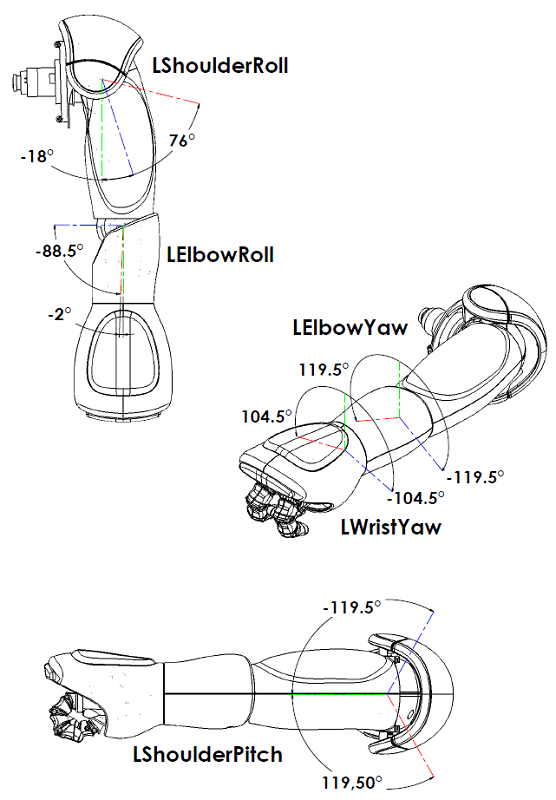
\includegraphics[width=\textwidth]{nao_diagrams/hardware_larmjoint_3.3.png}
\caption{Figure showing left arm}
\label{fig:nao_arm_joints_left1}
\end{figure}

\begin{figure}
\centering
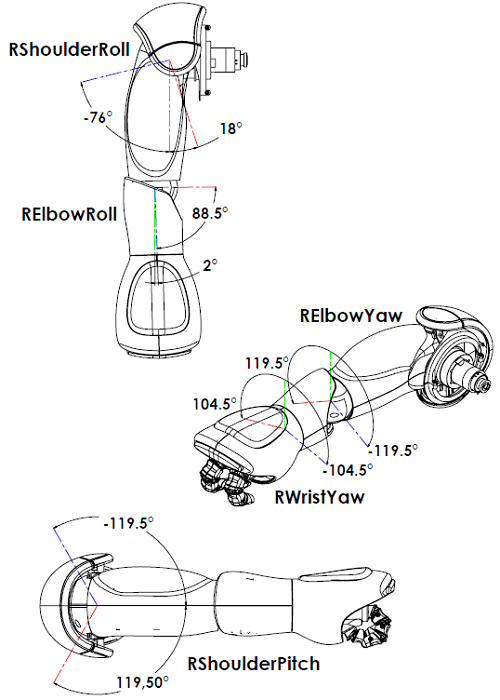
\includegraphics[width=\textwidth]{nao_diagrams/hardware_rarmjoint_3.3.png}
\caption{Figure showing right arm}
\label{fig:nao_arm_joints_right1}
\end{figure}

\begin{figure}
\centering
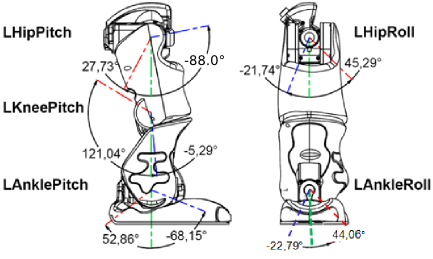
\includegraphics[width=\textwidth]{nao_diagrams/hardware_llegjoint.png}
\caption{Figure showing left leg}
\label{fig:nao_leg_joints_left1}
\end{figure}

\begin{figure}
\centering
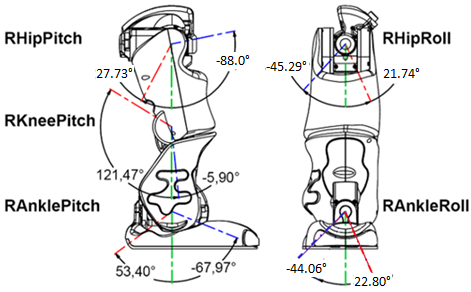
\includegraphics[width=\textwidth]{nao_diagrams/hardware_rlegjoint.png}
\caption{Figure showing right leg}
\label{fig:nao_leg_joints_right1}
\end{figure}

\begin{figure}
\centering
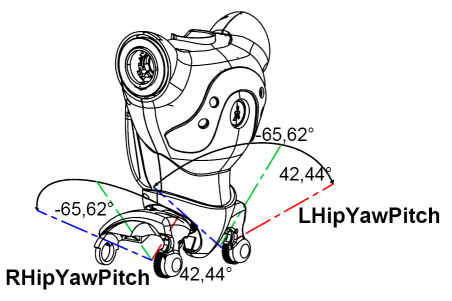
\includegraphics[width=\textwidth]{nao_diagrams/hardware_pelvisjoint.png}
\caption{Figure showing hip yaw-pitch}
\label{fig:nao_hip_yawpitch1}
\end{figure}


Need diagram showing arm symmetry for crawl results. 
\begin{figure}
\centering
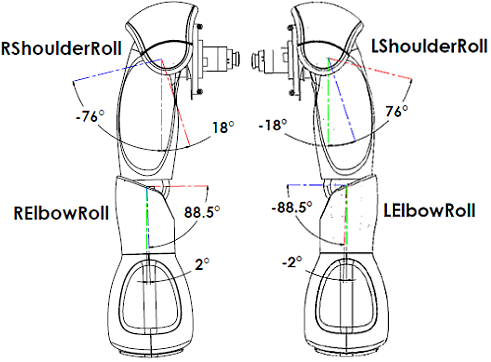
\includegraphics[width=\textwidth]{hardware_r_and_l_armjoint.png}
\caption{Figure showing arm joints and how they are a reflection.}
\label{fig:nao_arm_joints_reflect1}
\end{figure}

Need diagram showing different postures for crawl results. 
\begin{figure}
\centerline{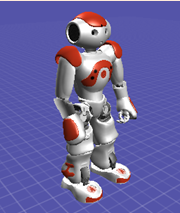
\includegraphics[width=0.33\textwidth]{posture/posture_stand.png}
            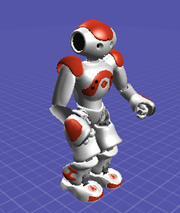
\includegraphics[width=0.33\textwidth]{posture/posture_standinit.png}
            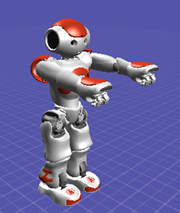
\includegraphics[width=0.33\textwidth]{posture/posture_standzero.png}
}
\vspace*{0.05in}
\centerline{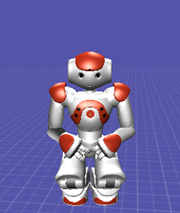
\includegraphics[width=0.33\textwidth]{posture/posture_crouch.png}
            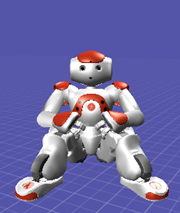
\includegraphics[width=0.33\textwidth]{posture/posture_sit.png}
            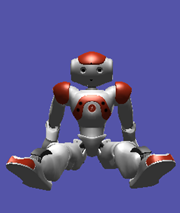
\includegraphics[width=0.33\textwidth]{posture/posture_sitrelax.png}
}
\vspace*{0.05in}
\centerline{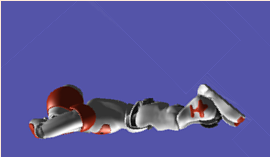
\includegraphics[width=0.5\textwidth]{posture/posture_lyingbelly.png}
            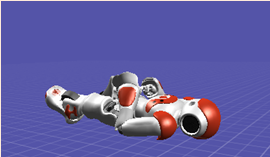
\includegraphics[width=0.5\textwidth]{posture/posture_lyingback.png}
}
\caption{Figure showing postures.}
\label{fig:nao_postures1}
\end{figure}

\subsection{Lidar Hardware}
Hokuyo is a Lidar. What's a Lidar? How does it work and what does it give you? 
{Diagrams explaining things like pictures of lidar outputs}

\begin{figure}
\centering
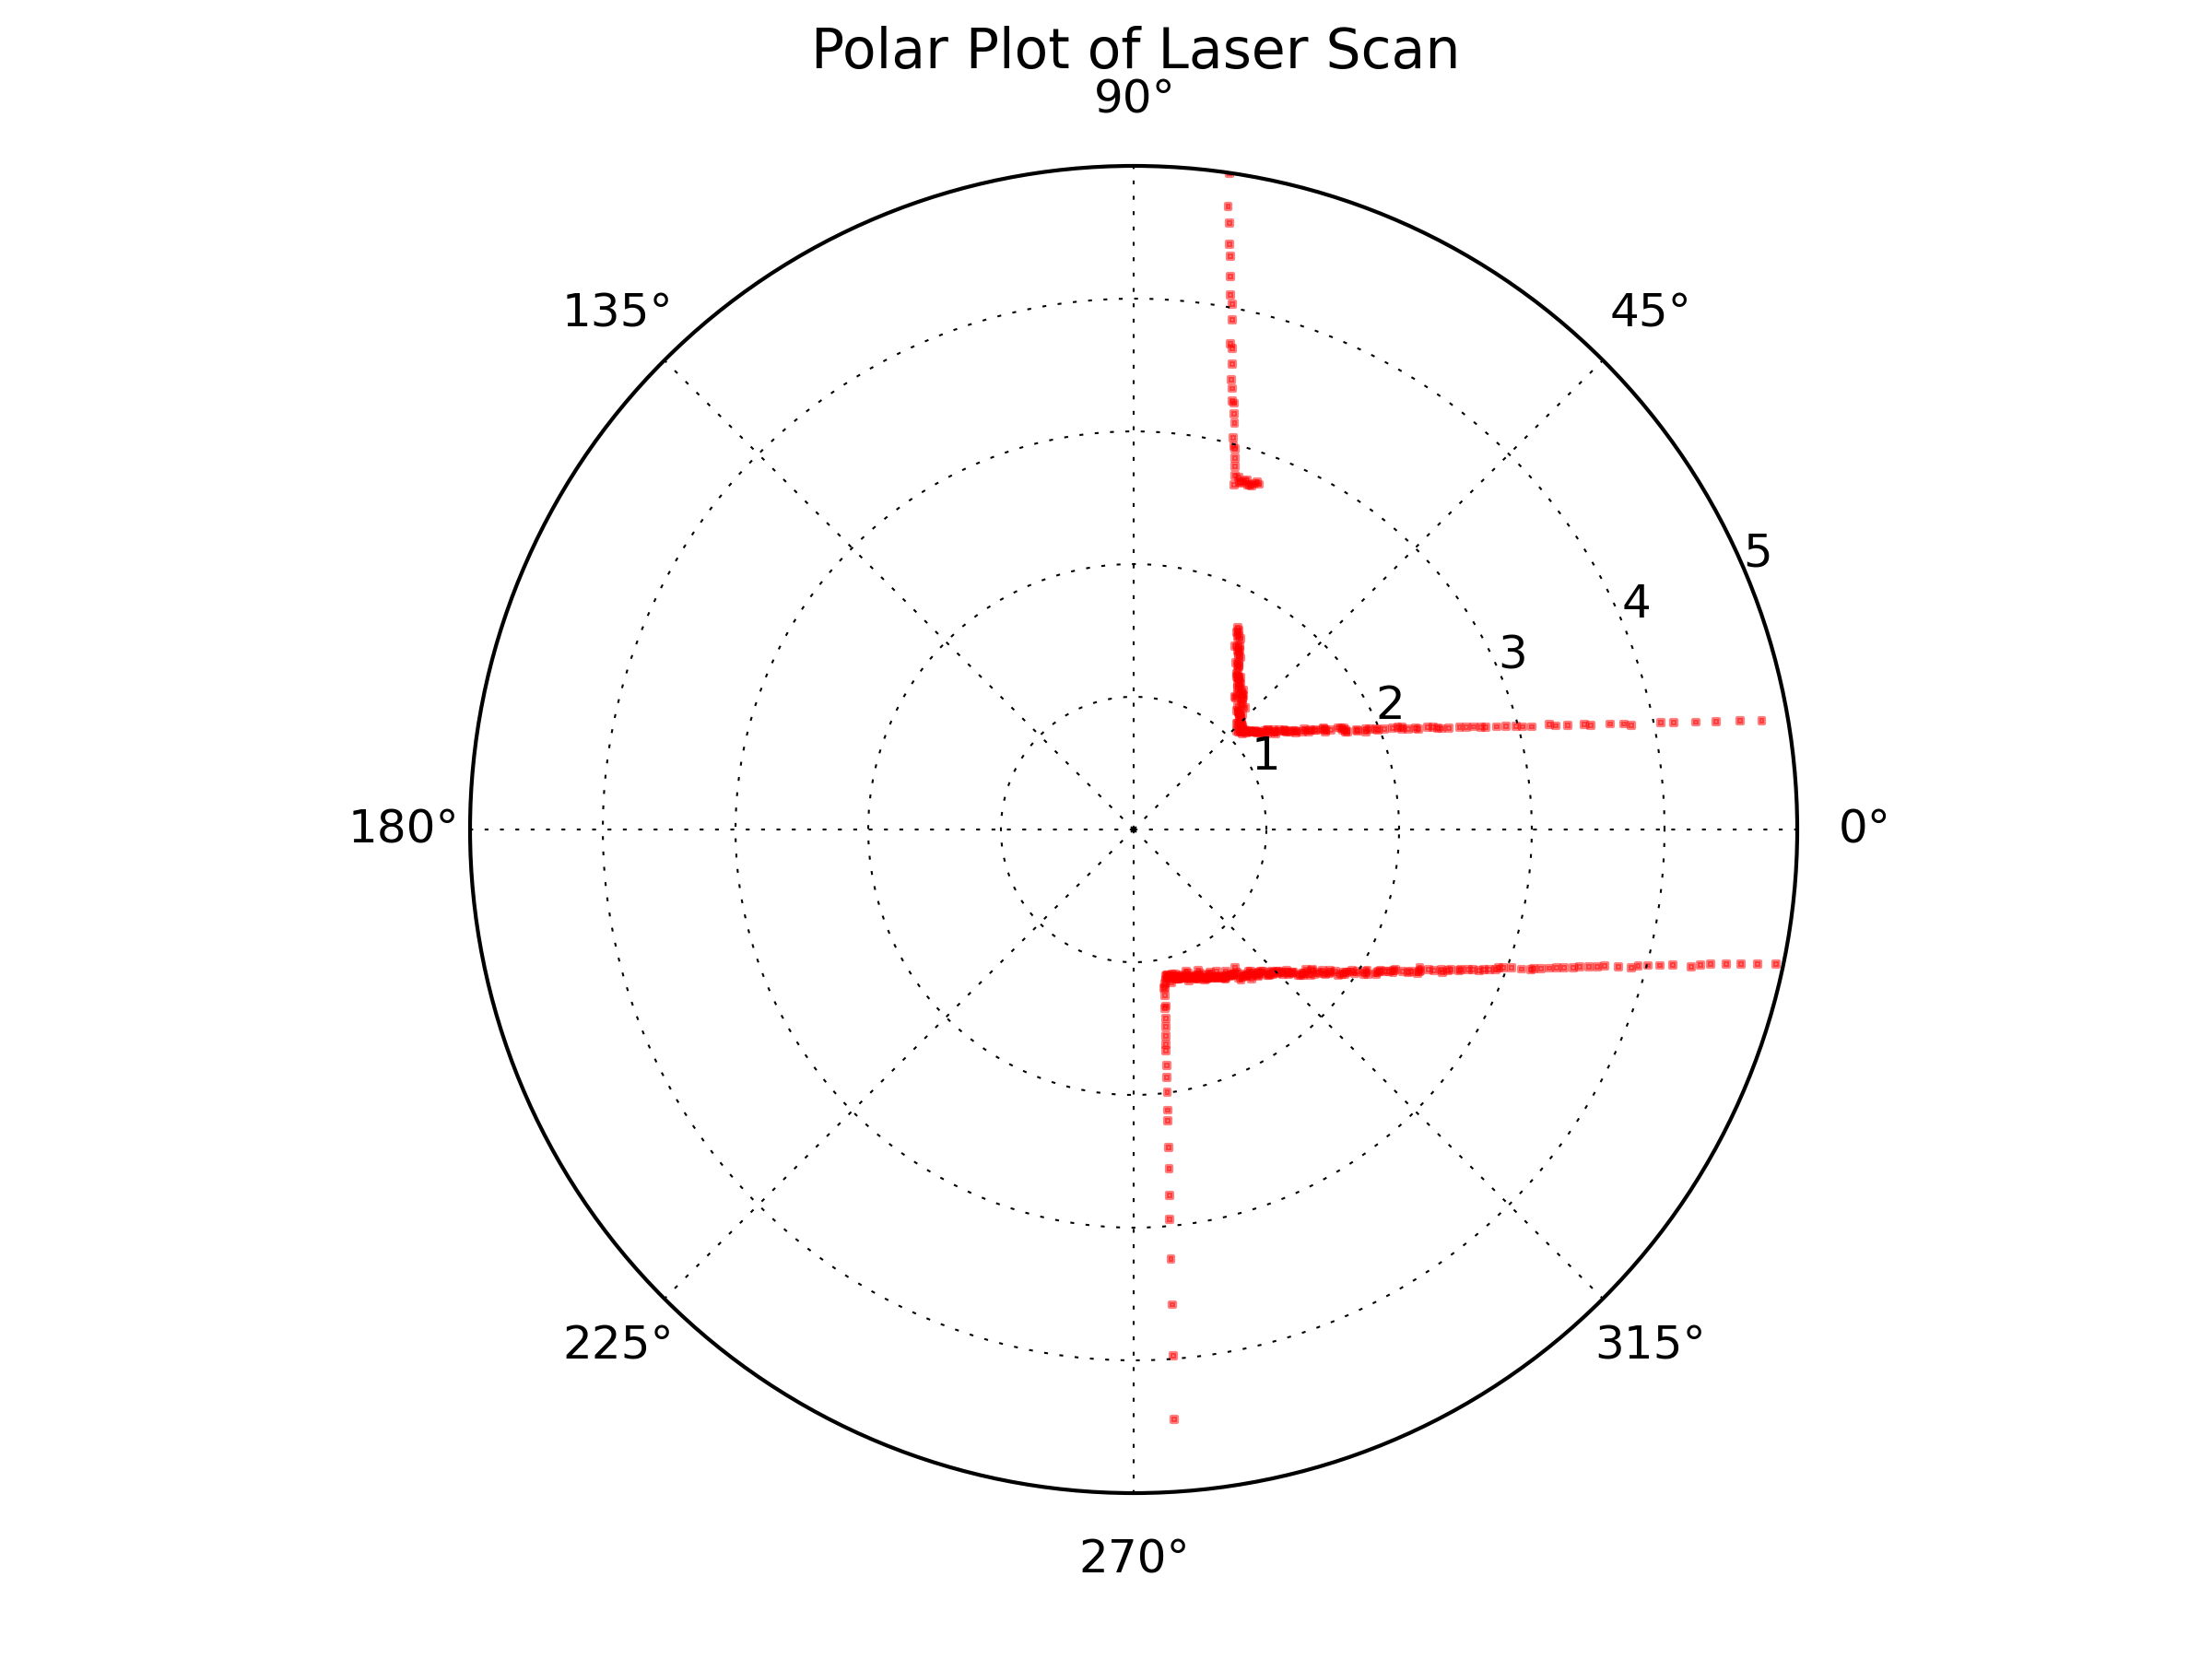
\includegraphics[height=0.4\textheight]{laser_scan_msg2.yaml_1.png}
\caption{Figure showing lidar scan, 5 meters like the URG\@.
         Robot is facing a hallway, to it's left is a doorway.}
\label{fig:lidar_scan1}
\end{figure}

Indoor only, not rated for outdoors.

USB 2.0


\begin{table}
\newcolumntype{R}{>{\raggedleft\arraybackslash}X}
%\centering
\begin{tabularx}{\textwidth}{|R||R|R|R|R|R|}
\hline
\textbf{Param}   &	\textbf{Condition} & \textbf{Min} & \textbf{Typ} & \textbf{Max} & \textbf{Units} \\	\hline\hline
View Angle 	         &                     &              & 240              &              & degrees        \\	\hline
Angular Resolution 	 & .                   & .            & 0.36             &  .           & degrees        \\	\hline
Range 	             &                     & 20           &                  & 4000         & mm             \\	\hline 
Linear Resolution    &  .                  & .            & 1                & .            & mm             \\	\hline 
Accuracy             & Distance 20 mm to 1000 mm &        & $\pm$ 30         &   .          & mm             \\	\hline 
%        	         & Distance 20 mm to 4000 mm &        & $\pm$ 3          &              & \%             \\	\hline 
%Update Rate	  & cond & min & 100 & max & ms/scan \\	\hline \hline
%Weight 	  & cond & min & 160 & max & g \\	\hline 
%Width 	  & cond & min & 240 & max & degrees \\	\hline 
%Length 	  & cond & min & 240 & max & degrees \\	\hline 
%Height	  & cond & min & 240 & max & degrees \\	\hline \hline
%Voltage Rating	  & cond & 4.75 & 5.0 & 5.25 & V \\	\hline 
%Current Consumption	  & cond & min & 500 & 800 & mA \\	\hline 
\end{tabularx} 
\caption{Things}
\label{tab:lidar_params1}
\end{table}


Here is where you get the information about the Lidar \cite{urg_specs}.

\begin{figure}
\centering
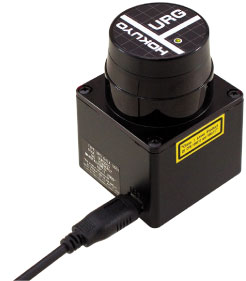
\includegraphics[height=0.4\textheight]{hokuyo/urg_04lx_ug01_top.jpg}
\caption{Figure showing Lidar.}
\label{fig:lidar_top1}
\end{figure}

\begin{figure}
\centering
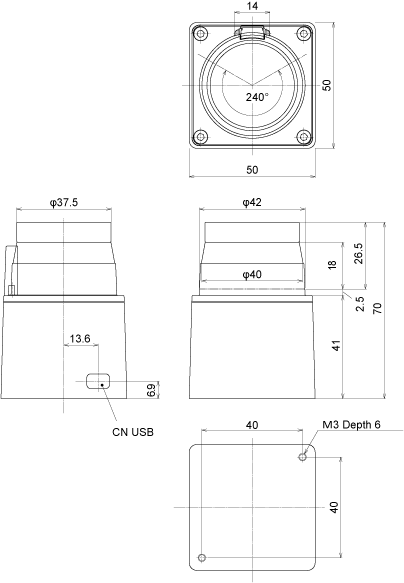
\includegraphics[height=0.4\textheight]{hokuyo/urg_04lx_ug01_ed.png}
\caption{Figure showing Lidar.}
\label{fig:lidar_diagram1}
\end{figure}

[Image showing angular and distance range of lidar.]



\subsection{Lidar Mount}
Design reqs: needed to rigidly attach to Nao for data transformation purposes, needed to see forward,
needed to be able to crawl with it, lightweight, Nao needed to be able to move his head while wearing it,
needed to be able to use the sonars (just in case).

Mounting it to the head seemed like it was going to be tough, so a vest was designed.
Straps and foam seemed like they'd hold well enough. In fact they hold so well I can lift Nao up by the mount.
[Show Solidworks design.]
\begin{figure}
\centering
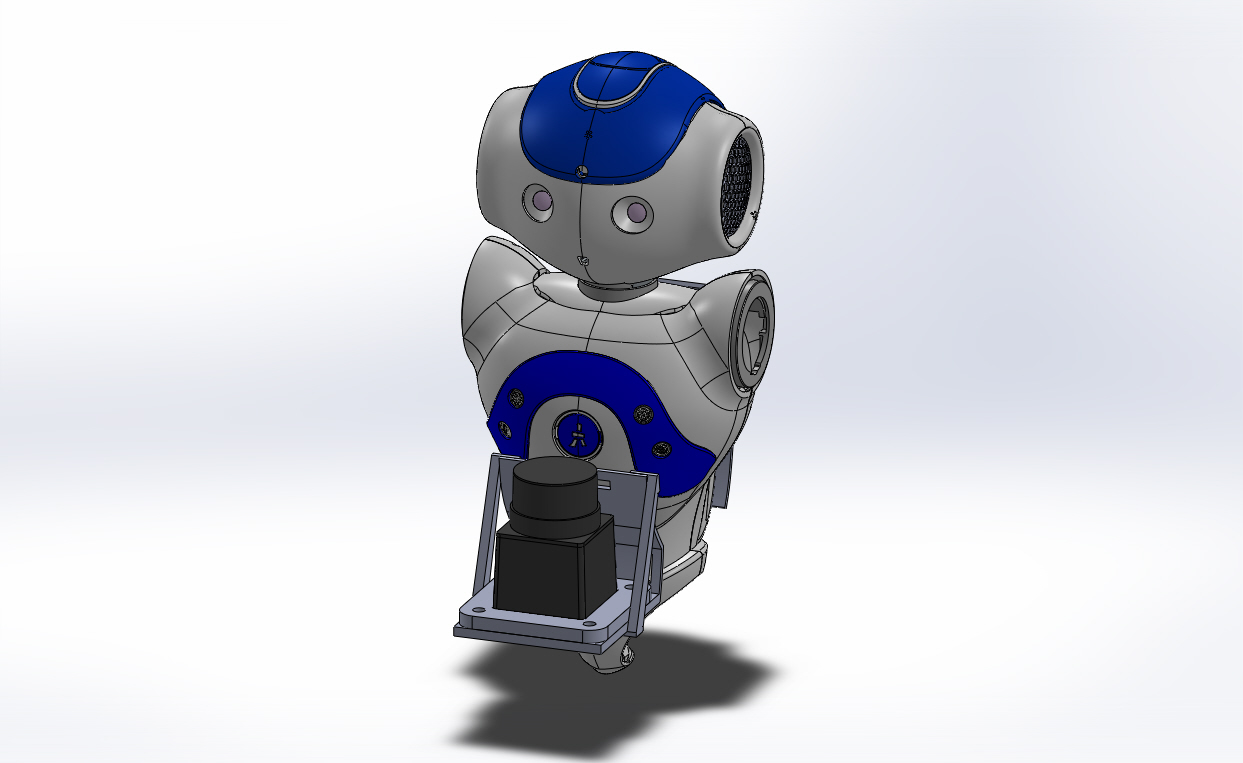
\includegraphics[height=0.4\textheight]{backpack/Assem_Nao_Dimetric1.jpg}
\caption{Figure showing assembled Nao Lidar.}
\label{fig:nao_lidar_mount_nao_dimetric1}
\end{figure}

\begin{figure}
\centering
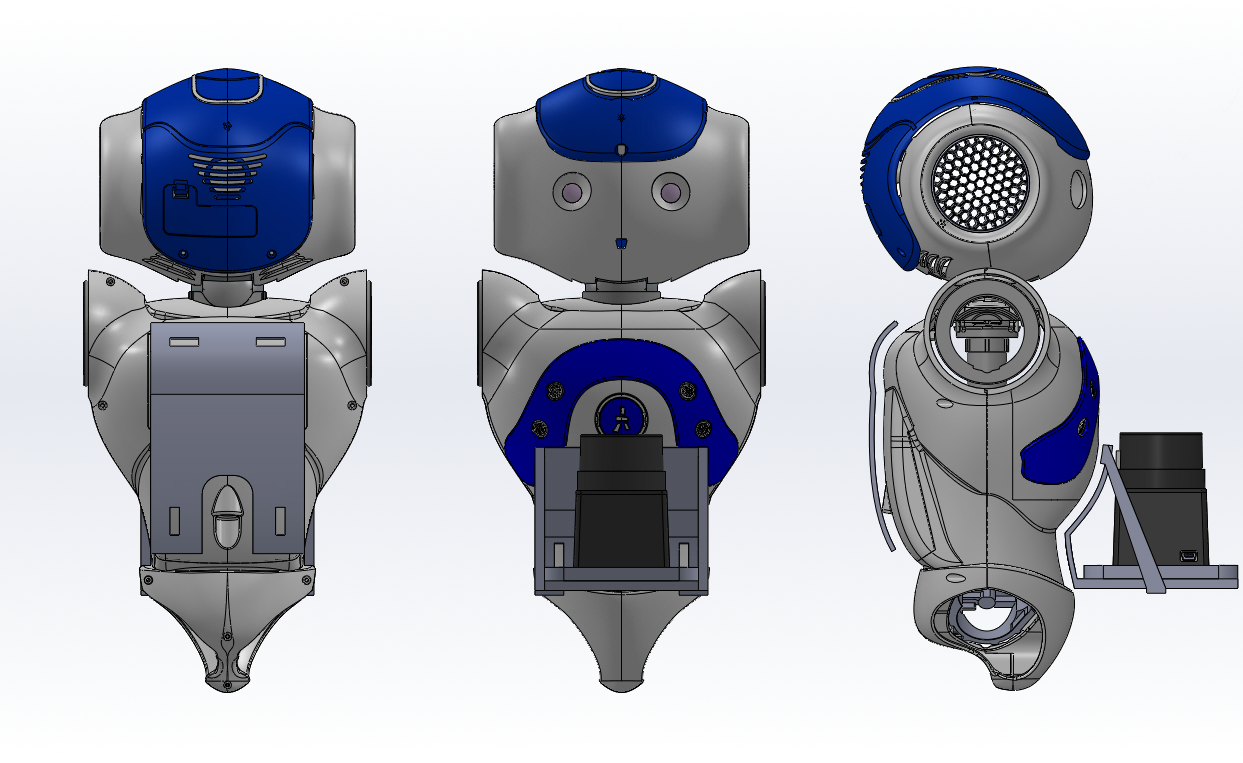
\includegraphics[height=0.4\textheight]{backpack/Assem_Nao_Three_View1.png}
\caption{Figure showing assembled Nao Lidar.}
\label{fig:nao_lidar_mount_nao_three_view1}
\end{figure}

\begin{figure}
\centering
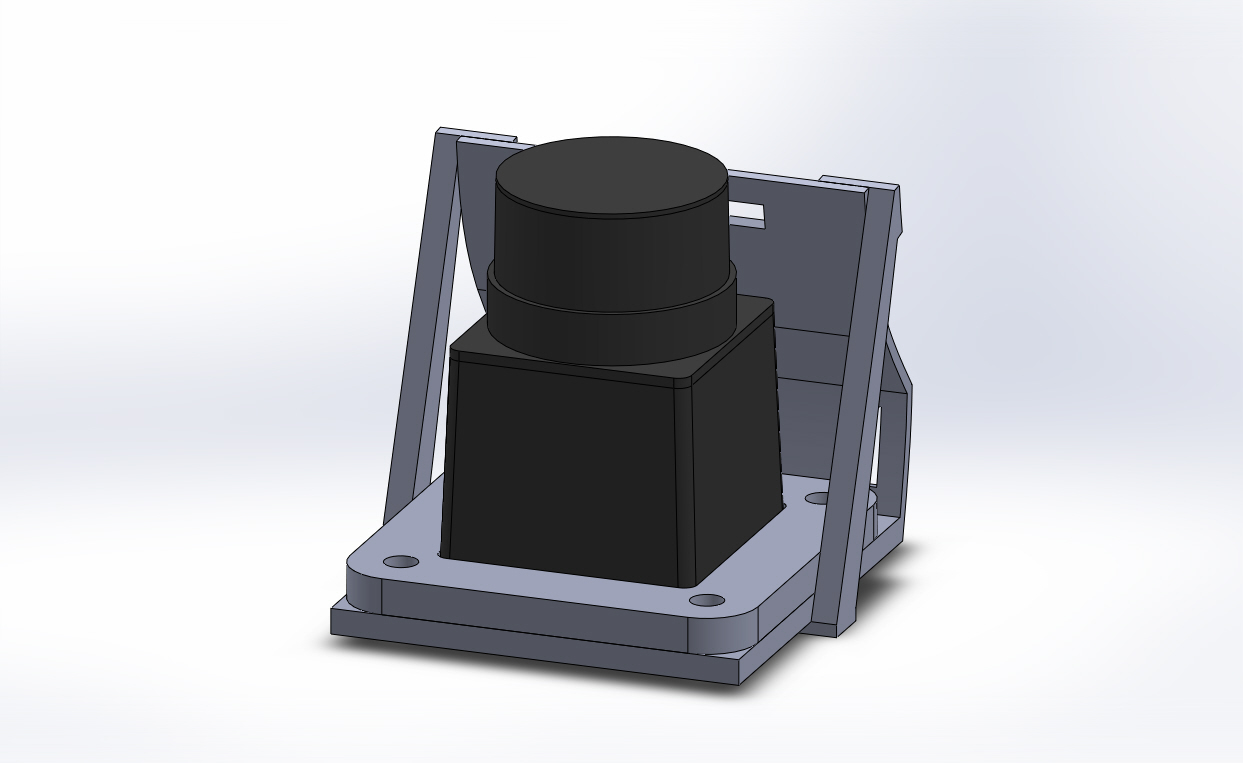
\includegraphics[height=0.4\textheight]{backpack/Assem_FrontOnly_Dimetric1.jpg}
\caption{Figure showing assembled Nao Lidar.}
\label{fig:nao_lidar_mount_dimetric1}
\end{figure}

\begin{figure}
\centering
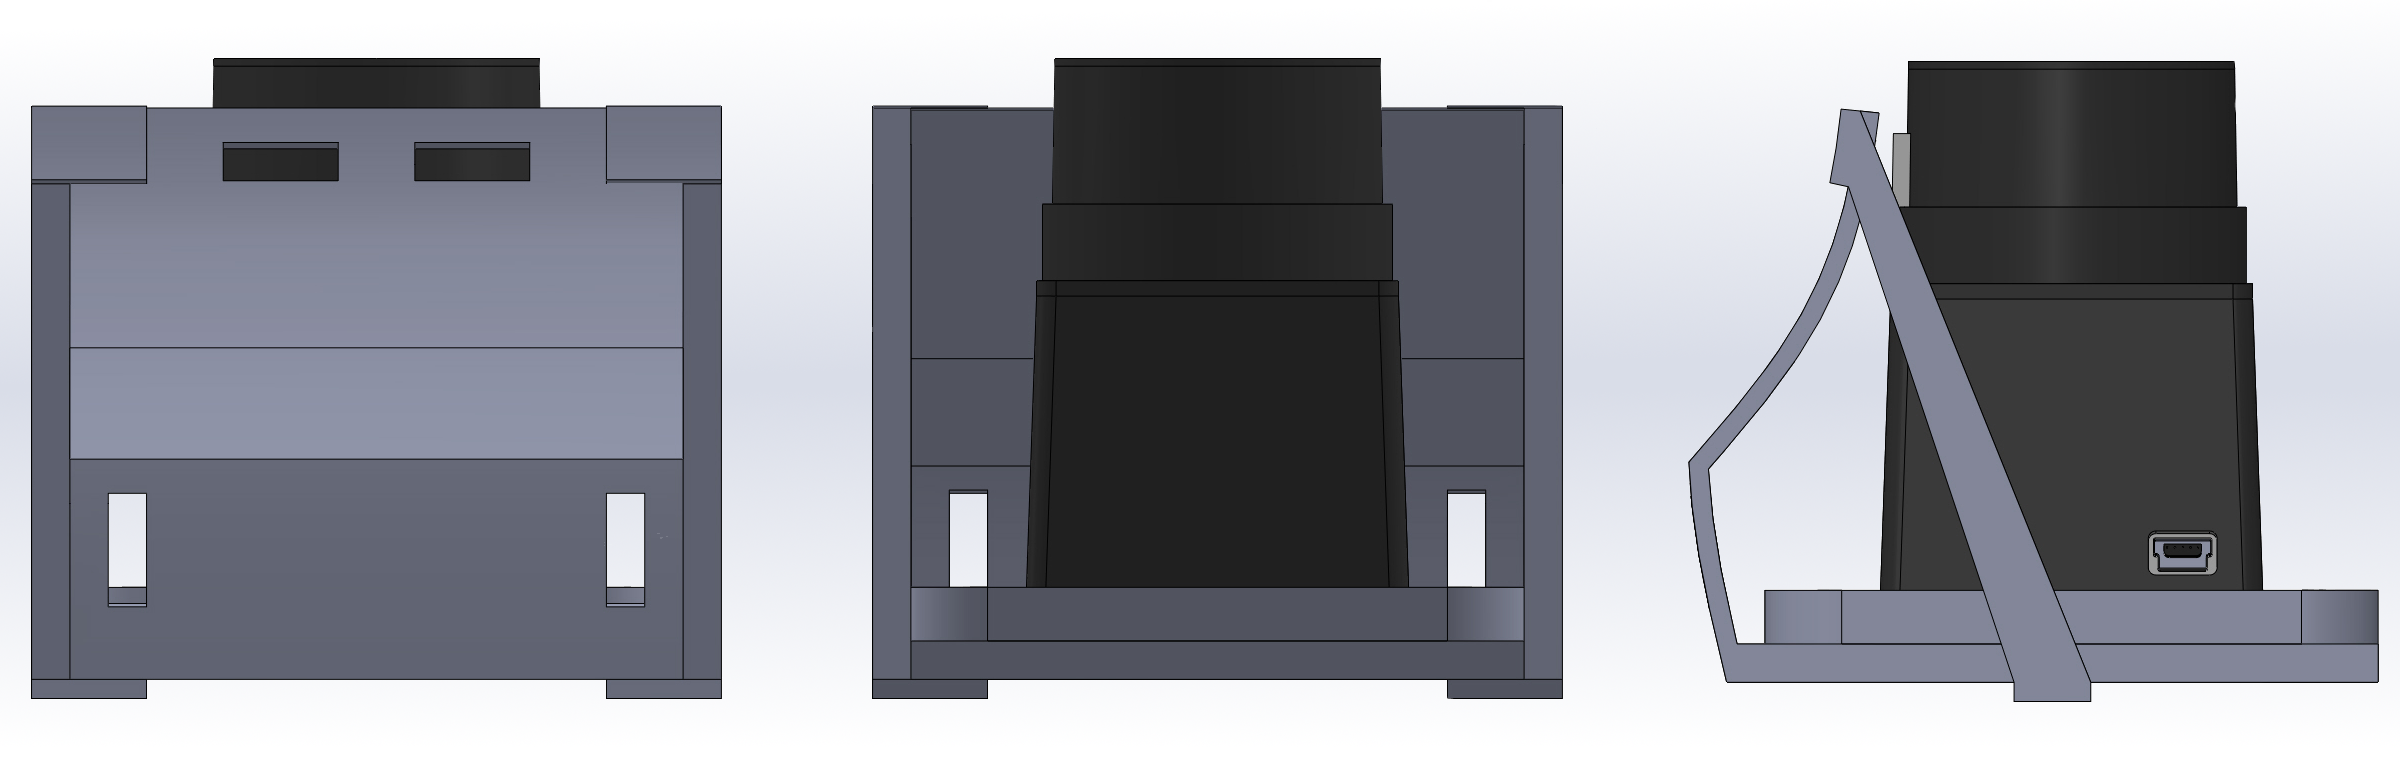
\includegraphics[width=\textwidth]{backpack/Assem_FrontOnly_Three_View1.png}
\caption{Figure showing assembled Nao Lidar.}
\label{fig:nao_lidar_mount_three_view1}
\end{figure}

\begin{figure}
\centering
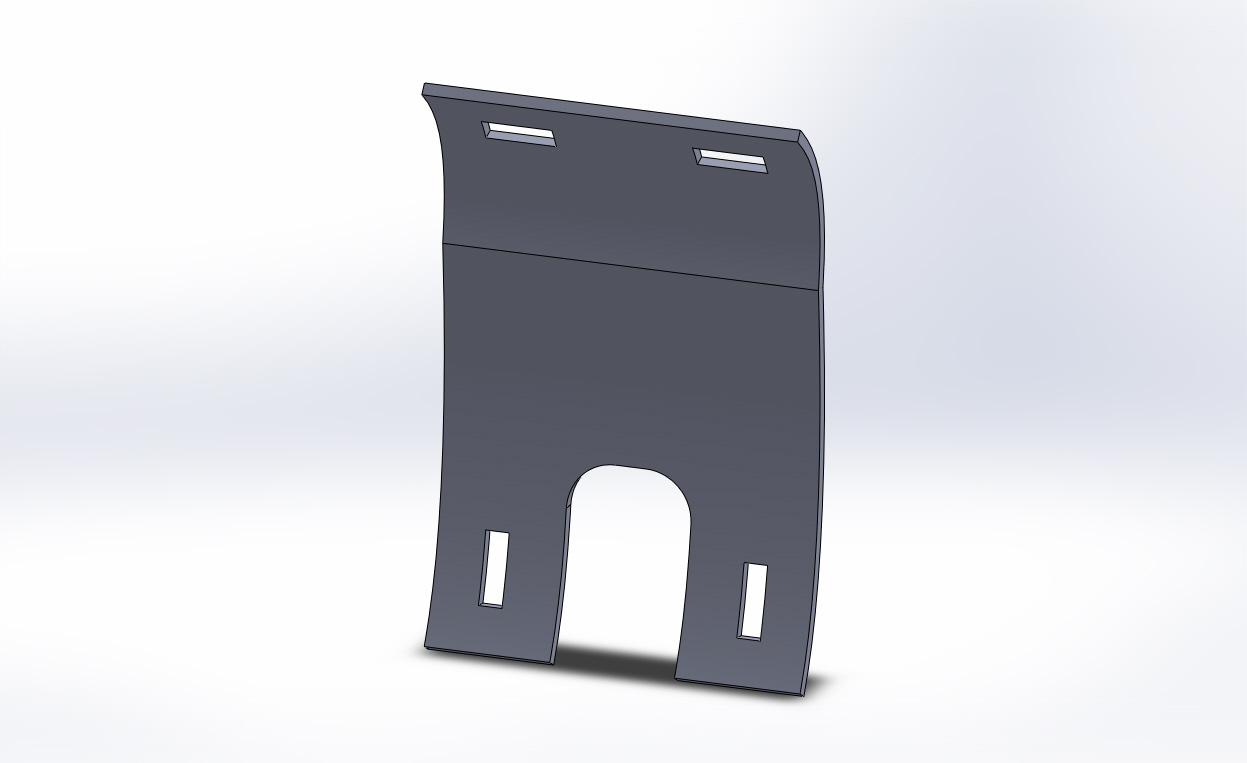
\includegraphics[height=0.4\textheight]{backpack/Back_Plate_Dimetric1.jpg}
\caption{Figure showing assembled Nao Lidar.}
\label{fig:nao_lidar_mount_backplate_dimetric1}
\end{figure}

\begin{figure}
\centering
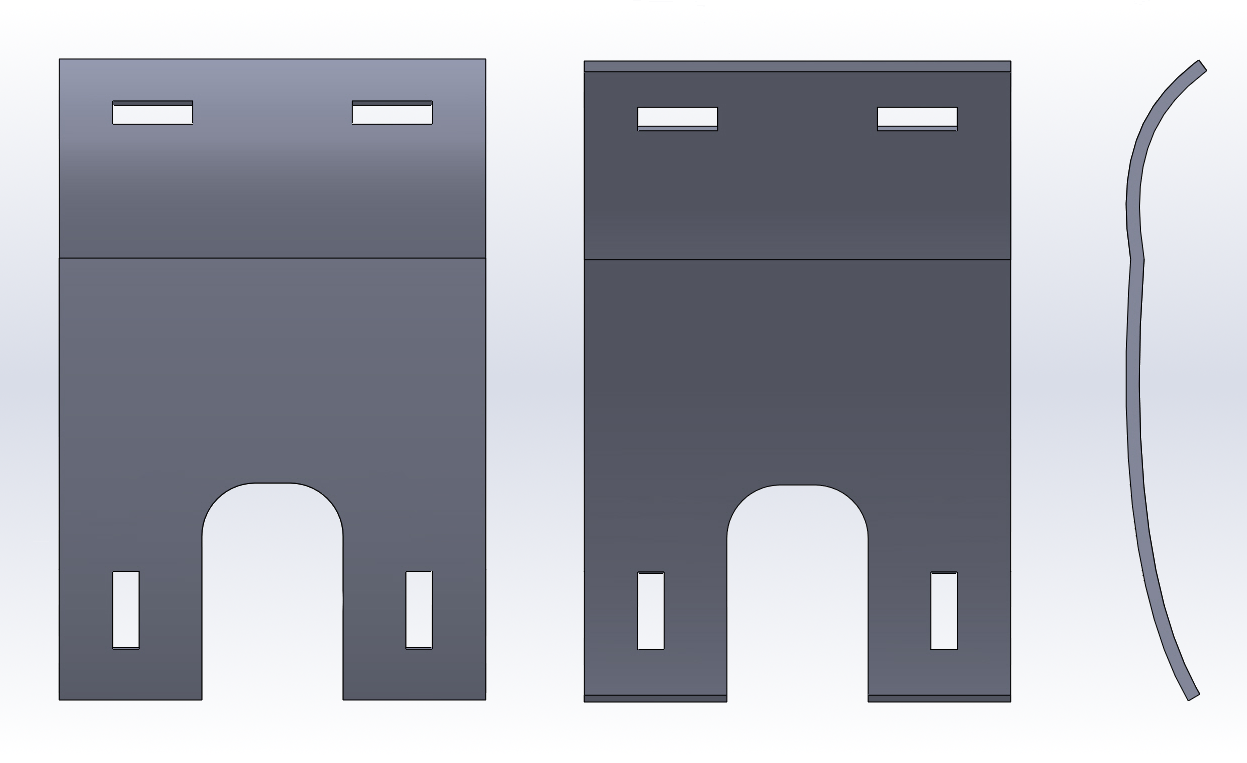
\includegraphics[width=\textwidth]{backpack/Back_Plate_Three_View1.png}
\caption{Figure showing assembled Nao Lidar.}
\label{fig:nao_lidar_mount_backplate_three_view1}
\end{figure}

\begin{figure}
\centering
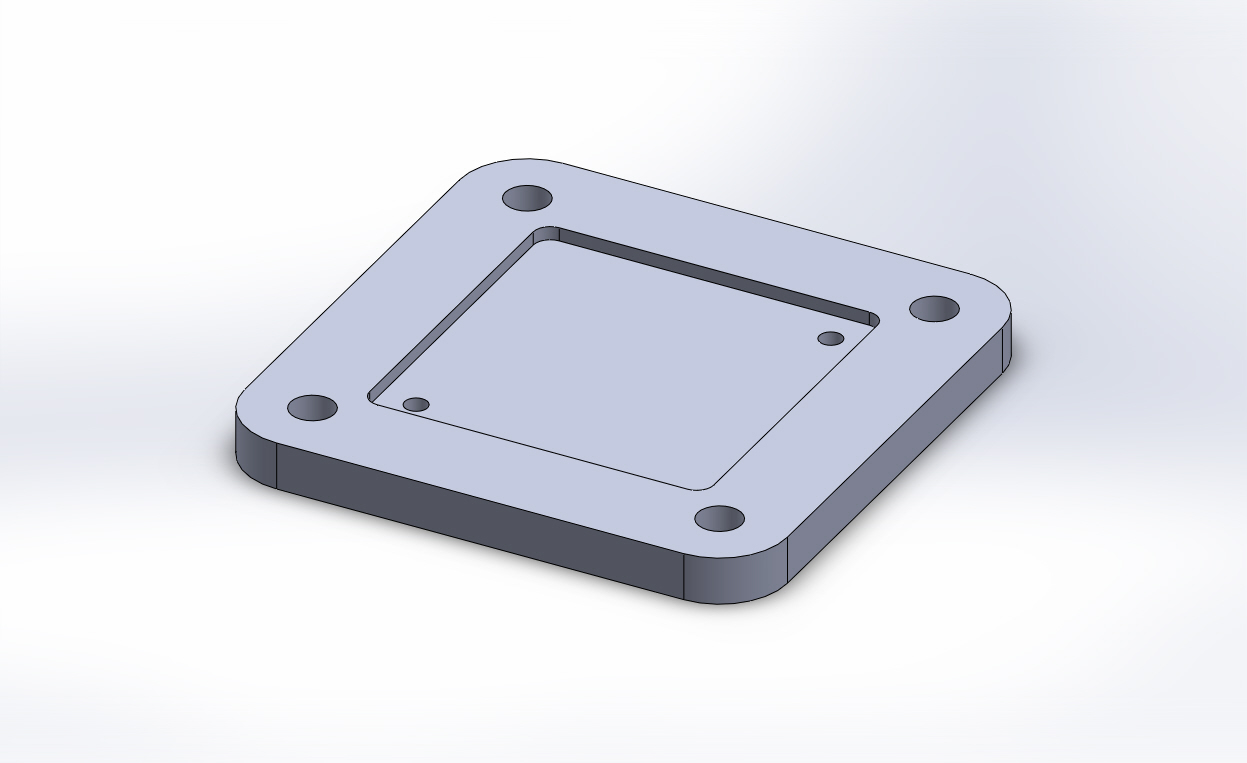
\includegraphics[height=0.4\textheight]{backpack/Base_Plate_Trimetric1.jpg}
\caption{Figure showing assembled Nao Lidar.}
\label{fig:nao_lidar_mount_baseplate_trimetric1}
\end{figure}

\begin{figure}
\centering
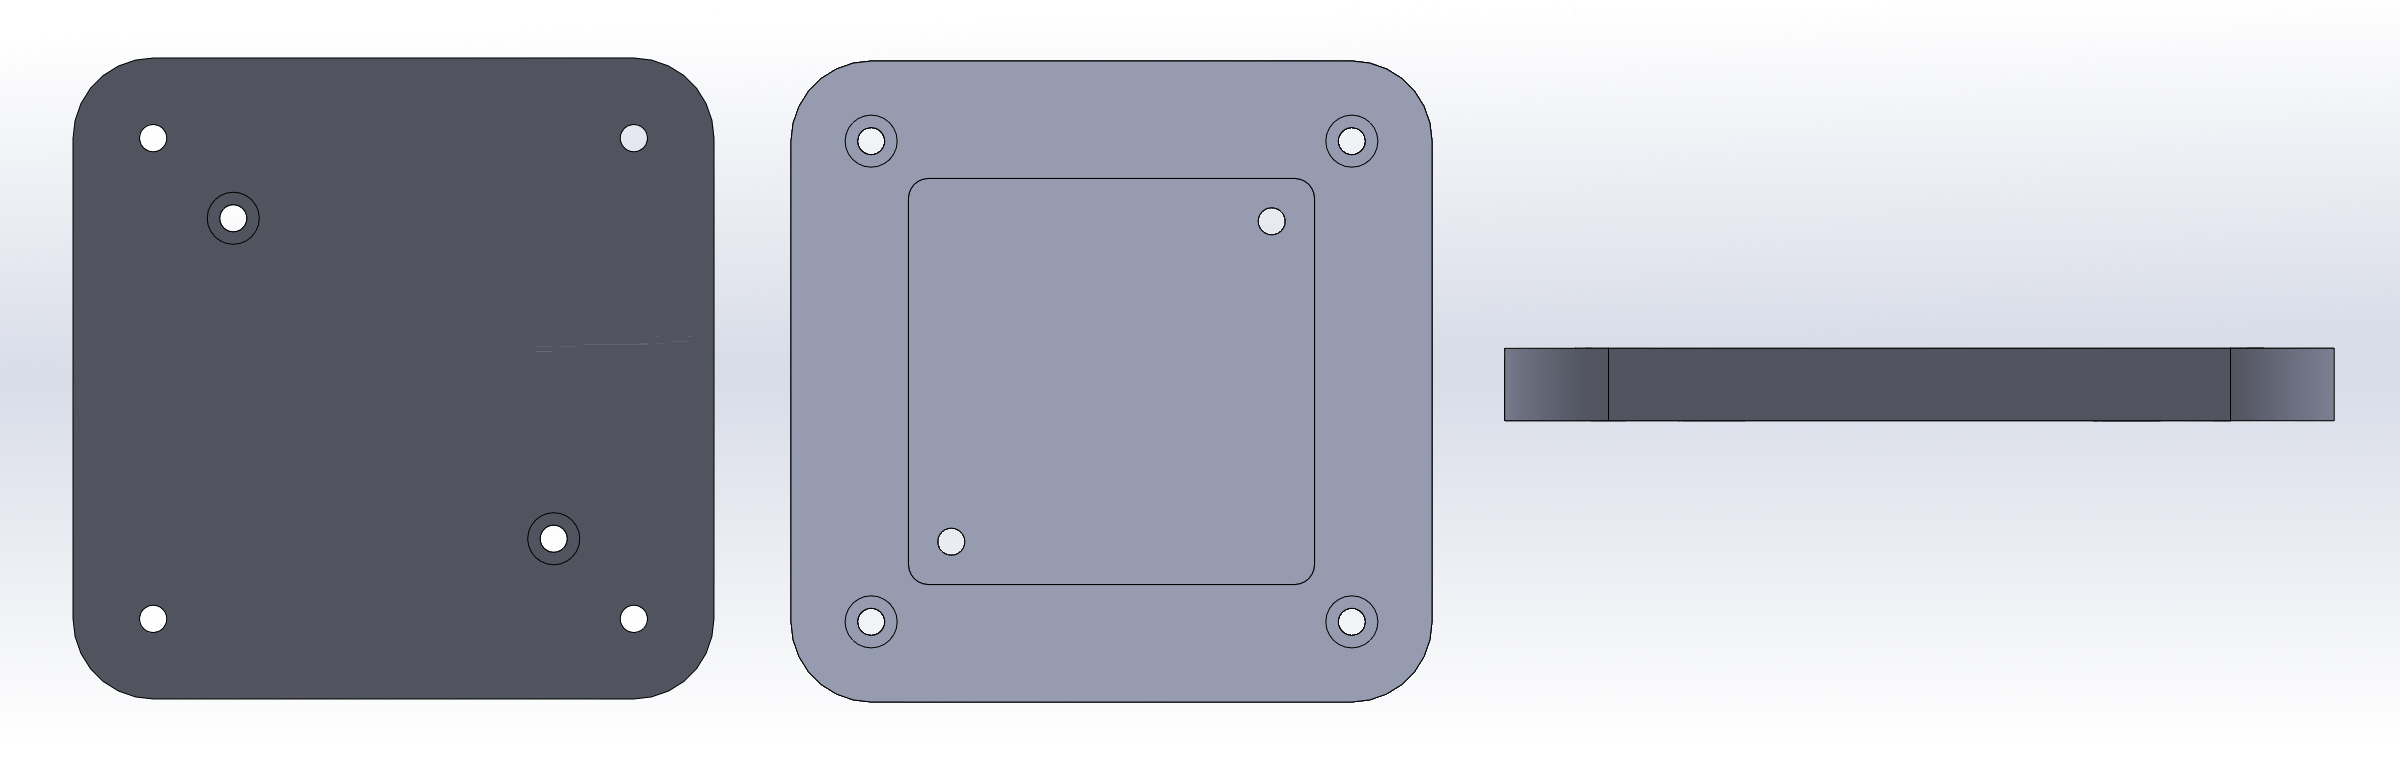
\includegraphics[width=\textwidth]{backpack/Base_Plate_Three_View1.png}
\caption{Figure showing assembled Nao Lidar.}
\label{fig:nao_lidar_mount_baseplate_three_view1}
\end{figure}

\begin{figure}
\centering
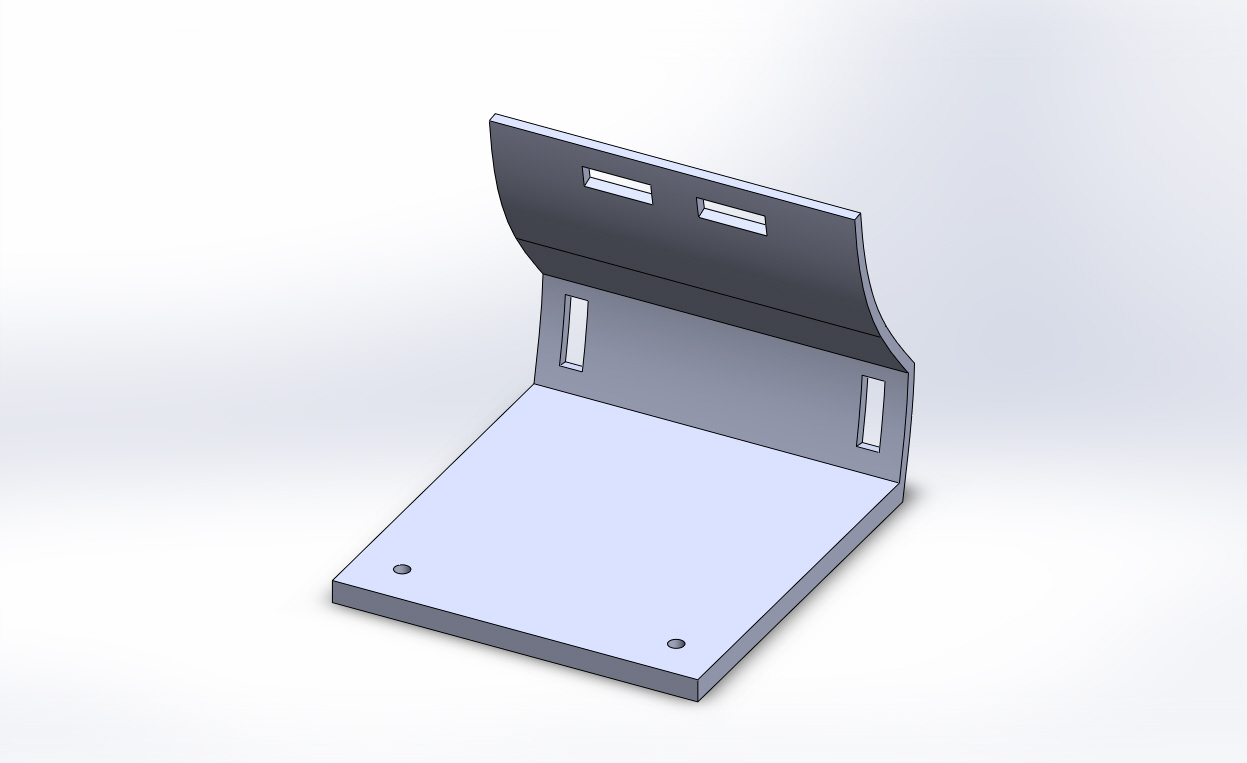
\includegraphics[height=0.4\textheight]{backpack/Front_Plate_Trimetric1.jpg}
\caption{Figure showing assembled Nao Lidar.}
\label{fig:nao_lidar_mount_frontplate_trimetric1}
\end{figure}

\begin{figure}
\centering
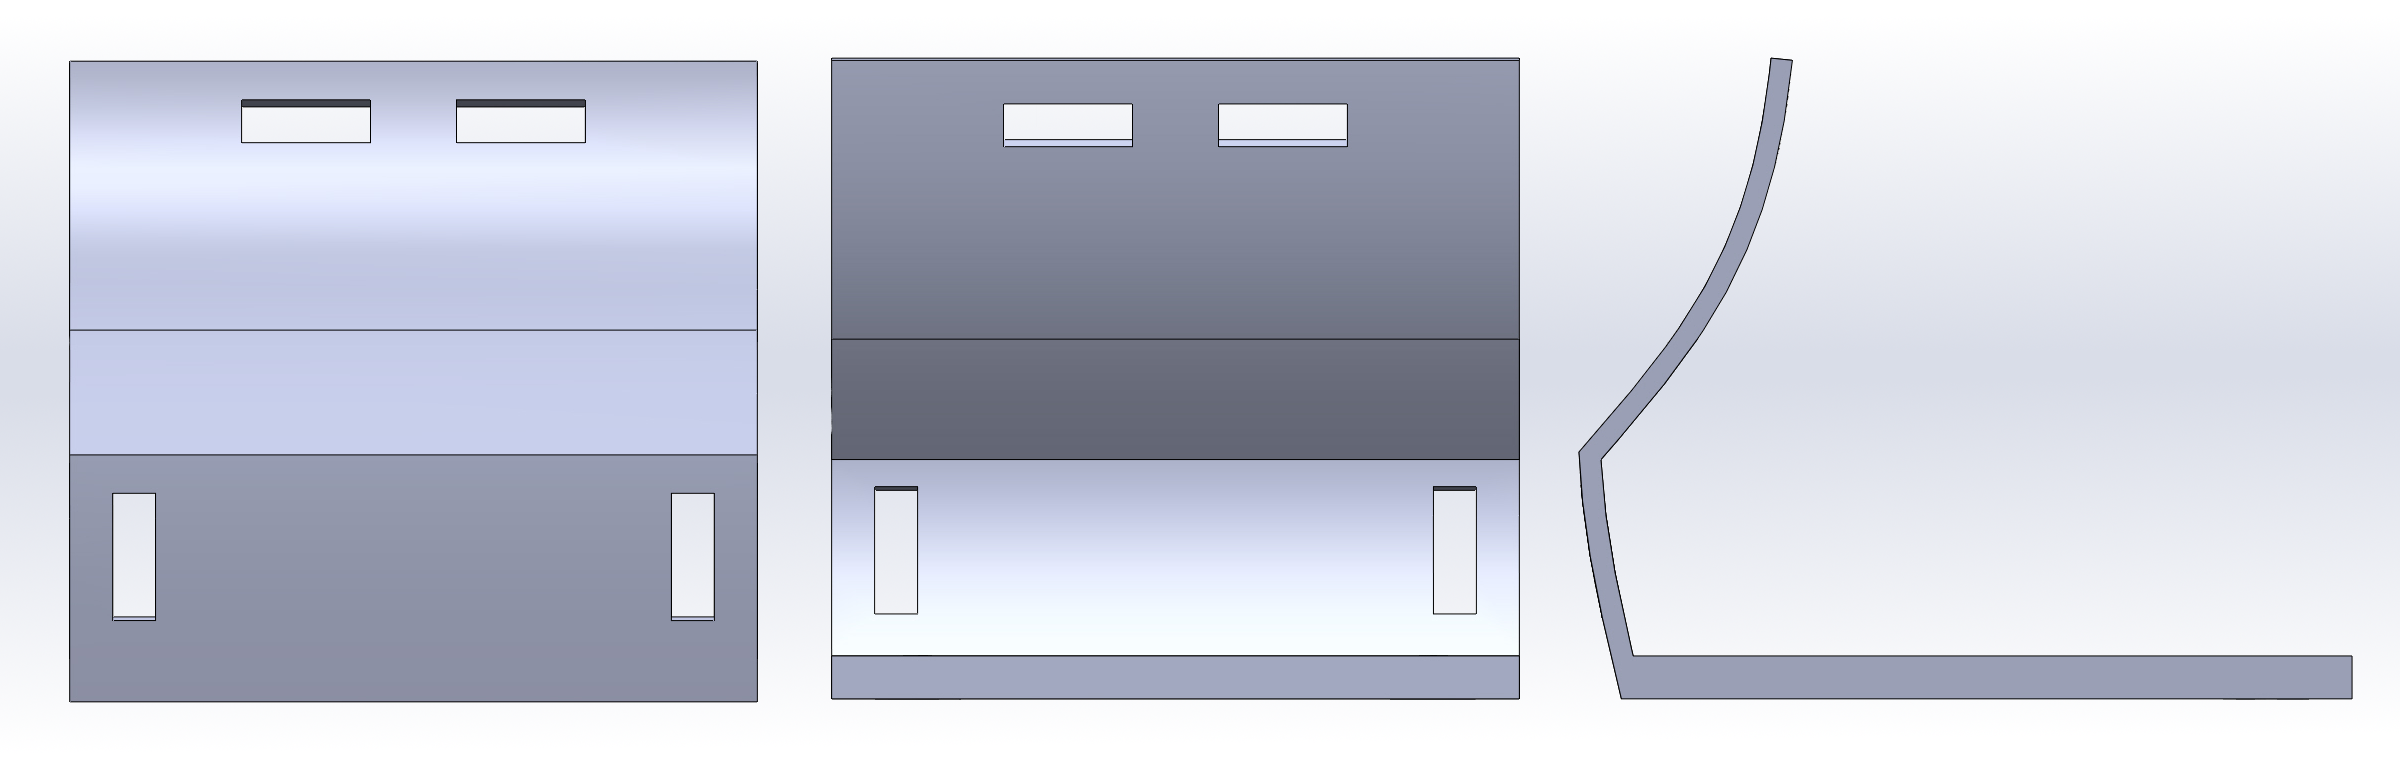
\includegraphics[width=\textwidth]{backpack/Front_Plate_Three_View1.png}
\caption{Figure showing assembled Nao Lidar.}
\label{fig:nao_lidar_mount_frontplate_three_view1}
\end{figure}

\begin{figure}
\centering
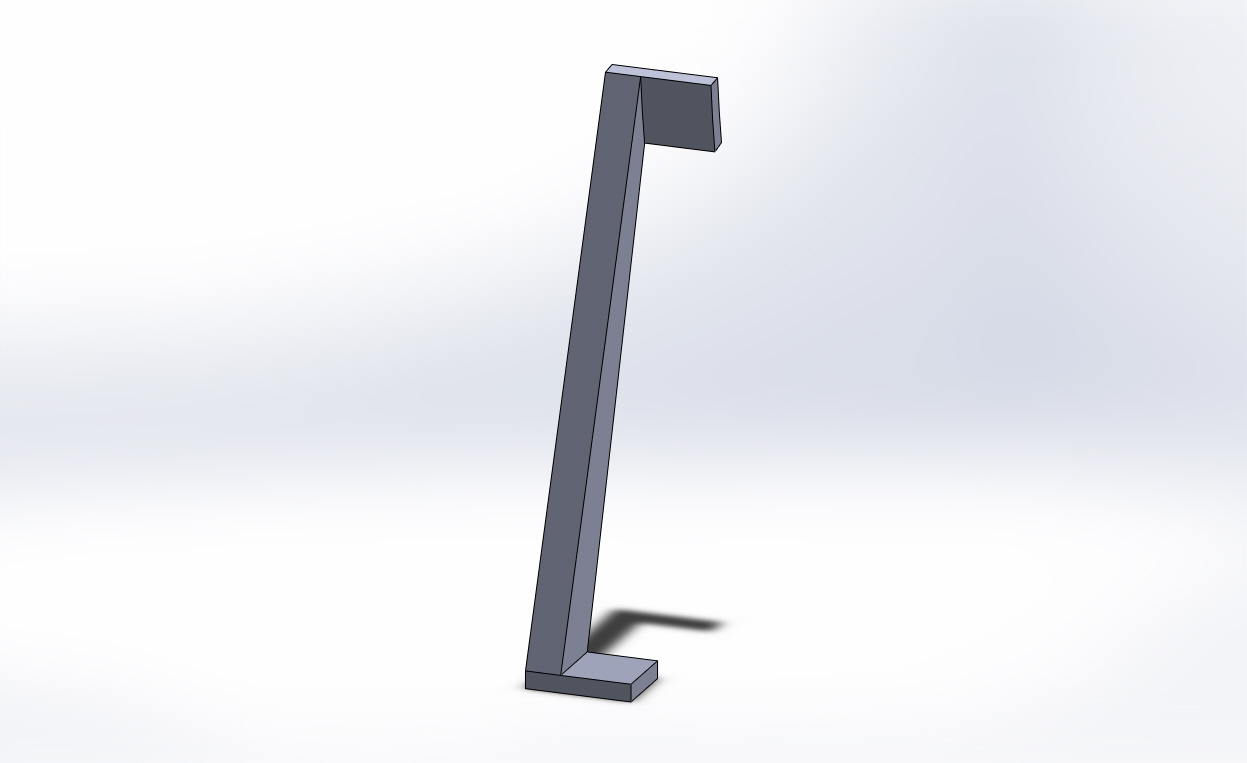
\includegraphics[height=0.4\textheight]{backpack/Support_Left_Trimetric1.jpg}
\caption{Figure showing assembled Nao Lidar.}
\label{fig:nao_lidar_mount_supportleft_trimetric1}
\end{figure}

\begin{figure}
\centering

\includegraphics[height=0.4\textheight]{backpack/Support_Left_Three_View1.jpg}
\caption{Figure showing assembled Nao Lidar.}
\label{fig:nao_lidar_mount_supportleft_three_view1}
\end{figure}

